\documentclass[utf8,9pt]{beamer}
\usepackage[T1]{fontenc}
\usepackage[italian]{babel}

\usefonttheme{professionalfonts}
\usepackage{kpfonts,booktabs,particlessymb,siunitx}
\usepackage[font=scriptsize,labelformat=empty]{caption}

\sisetup{per-mode=symbol,
  inter-unit-separator={}\cdot{},
  exponent-product=\cdot,
  output-product=\cdot,
  separate-uncertainty=true
}

\title{Raggi cosmici}
\author{Mosè Giordano}
\date{XX aprile 2013}
\institute[UniSalento]{Università del Salento}
\logo{
\includegraphics[width=10mm]{logo-unisalento}}
\usetheme{Madrid}
\useoutertheme[right]{sidebar}
\setbeamercovered{dynamic}
\usecolortheme{dove}

\begin{document}
\begin{frame}
  \maketitle
\end{frame}

\begin{frame}
  \frametitle{Piano della presentazione}
  \tableofcontents
\end{frame}

\section[Intro]{Introduzione}

% Per l'introduzione vedi l'articolo arXiv:1302.3307 e
% http://arstechnica.com/science/2013/02/supernova-observations-solve-the-mystery-of-cosmic-ray-origins/
% (questo può essere carino per l'inizio, parla della OMG particle)
\begin{frame}
  \frametitle{}
  
\end{frame}

\section[Fermi]{Fermi Gamma-ray Space Telescope}

\begin{frame}
  \frametitle{Fermi: obiettivi}
  \begin{figure}
    \centering
    % Fonte:
    % http://commons.wikimedia.org/wiki/File:Diagram_of_the_GLAST_instrument.jpg
    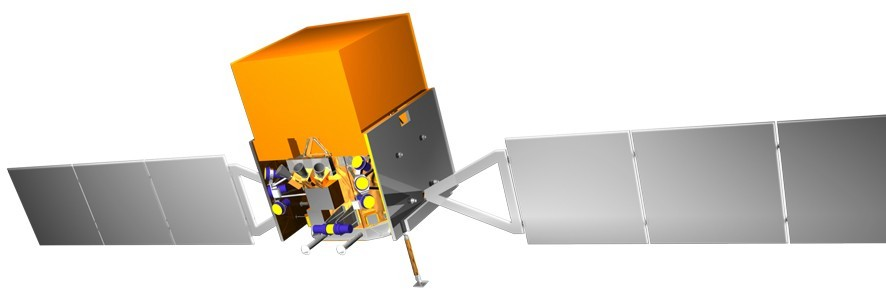
\includegraphics[width=0.5\columnwidth]{glast.jpg}
  \end{figure}
  Osservatorio per lo studio dei raggi gamma (da \SI{8}{\kilo\electronvolt} fino
  a oltre \SI{300}{\giga\electronvolt}) emessi da corpi celesti
  \begin{itemize}
  \item comprensione meccanismo di accelerazione particelle in AGN, pulsar e SNR
  \item studio sorgenti gamma non identificate e radiazione gamma diffusa
    galattica ed extra-galattica
  \item studio emissione ad altissima energia nei GRB
  \item rivelazione indiretta della materia oscura, attraverso suo decadimento o
    annichilazione in fotoni o elettroni e positroni
  \item osservazione evaporazione di MBH dalla presunta traccia di lampi gamma
  \end{itemize}
  È in orbita a \SI{550}{\kilo\metre} d'altezza dall'11 giugno 2008
\end{frame}

\begin{frame}
  \frametitle{Fermi: strumentazione}
  % Per approfondire vedi
  % http://www.nasa.gov/mission_pages/GLAST/spacecraft/index.html
  \begin{columns}
    \begin{column}{0.4\columnwidth}
      \begin{itemize}
      \item Large Area Telescope (LAT), sensibile alla radiazione gamma tra
        \SI{20}{\mega\electronvolt} e \SI{300}{\giga\electronvolt}
      \item Gamma-Ray Burst Monitor (GBM), studio di fenomeni transienti a
        energie relativamente più basse (tra \SI{8}{\kilo\electronvolt} e
        \SI{40}{\mega\electronvolt})
      \end{itemize}
    \end{column}
    \begin{column}{0.6\columnwidth}
      \begin{figure}
        \centering
        % Fonte: http://commons.wikimedia.org/wiki/File:GLAST_schematic.jpg
        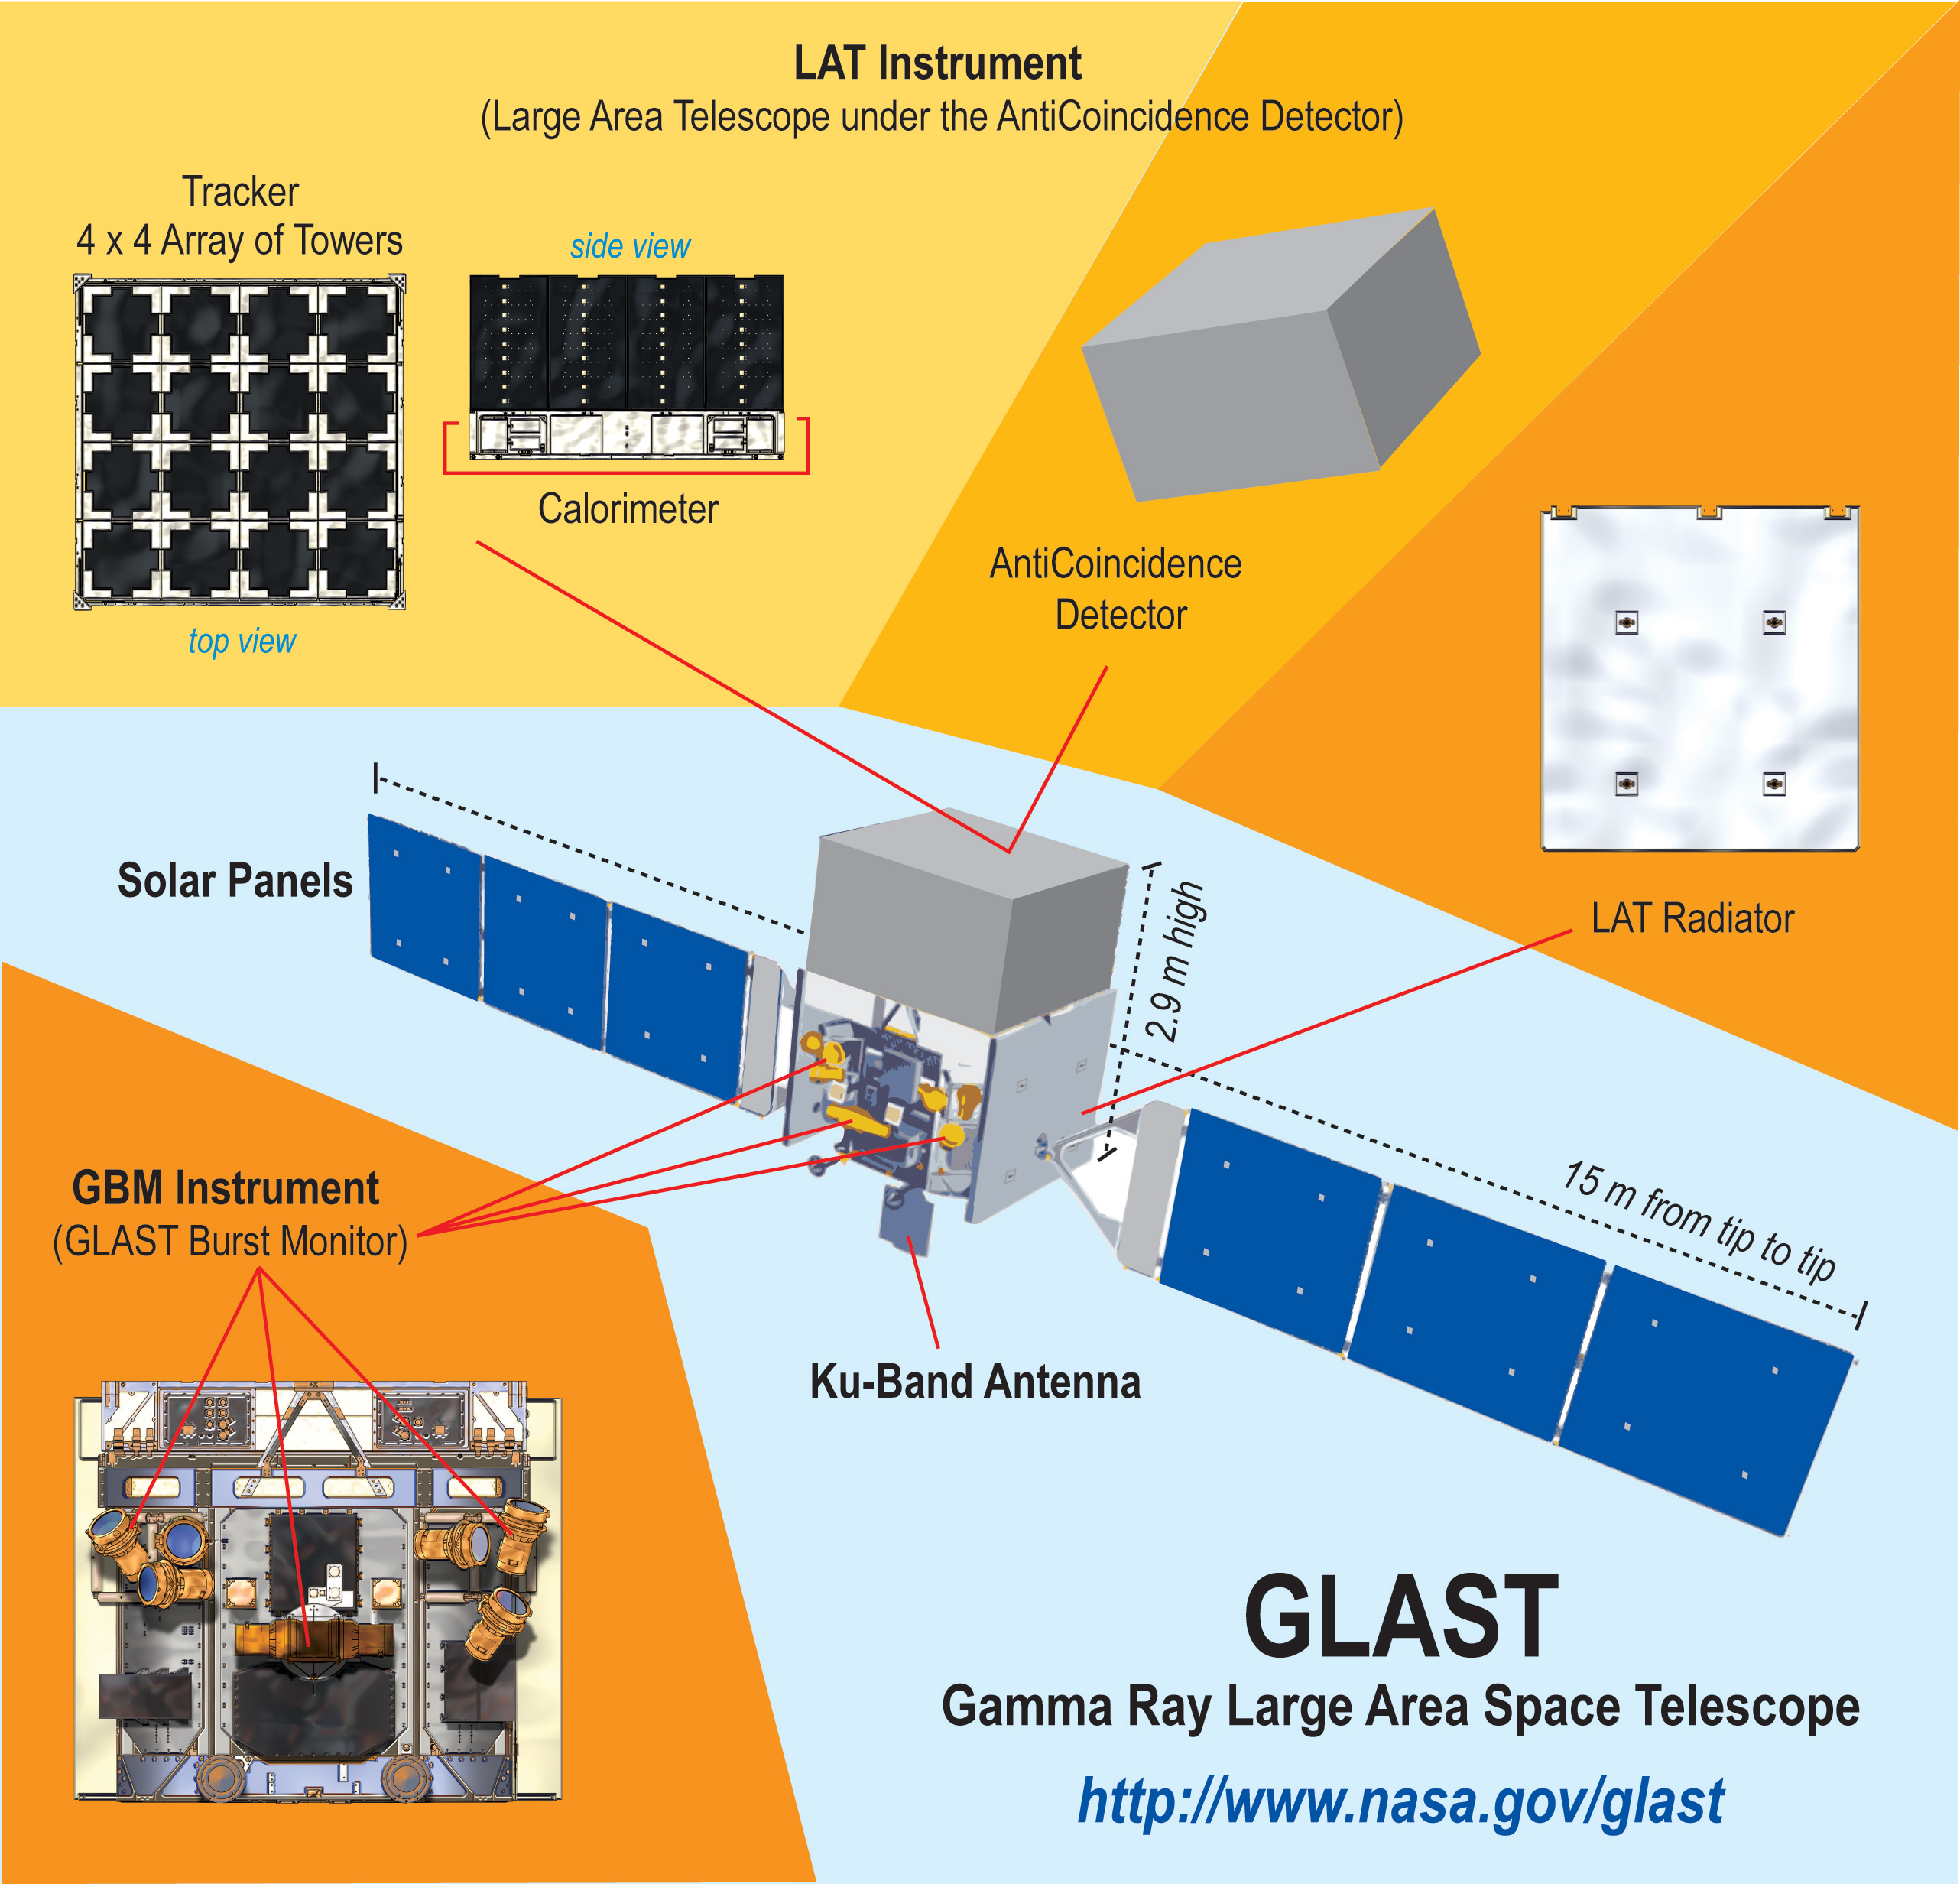
\includegraphics[width=\columnwidth]{glast_schematic.jpg}
      \end{figure}
    \end{column}
  \end{columns}
\end{frame}

\begin{frame}
  \frametitle{}
  \begin{figure}
    \centering
    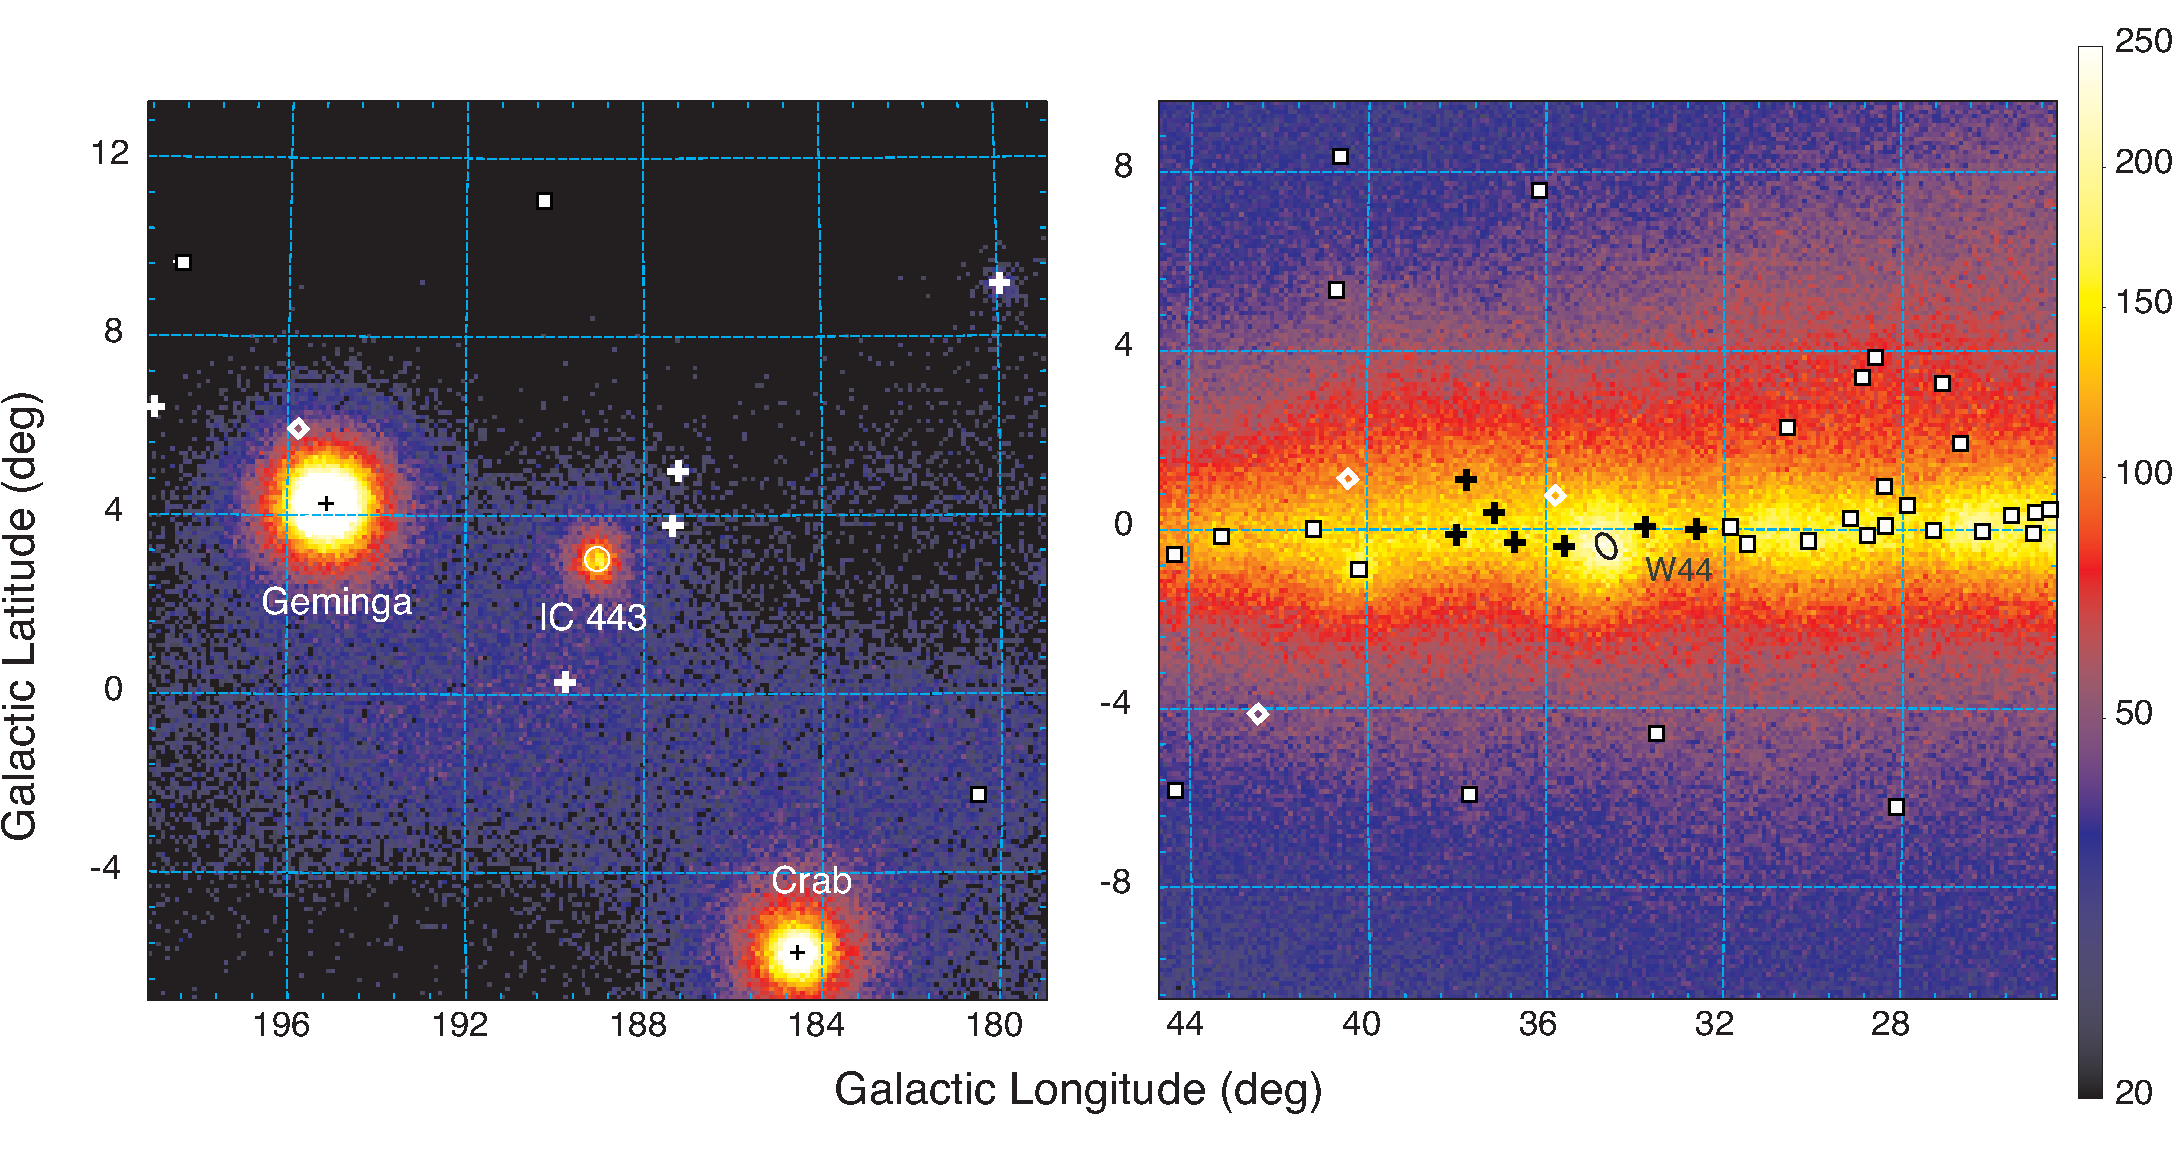
\includegraphics[width=0.8\columnwidth]{1231160fig1.pdf}
    \caption{Mappa del conteggio di raggi gamma in un campo di
      $\SI{20}{\degree} \times \SI{20}{\degree}$ attorno a IC 443 (sinistra) e
      W44 (destra) nell'intervallo di energia da \SI{60}{\mega\electronvolt} a
      \SI{2}{\giga\electronvolt}.}
  \end{figure}
\end{frame}

\section[AMS]{Alpha Magnetic Spectrometer}

\begin{frame}
  \frametitle{}
  
\end{frame}
\end{document}

%%% Local Variables:
%%% mode: latex
%%% TeX-master: t
%%% End:
